\documentclass[aspectratio=169]{beamer}
\usepackage{xcolor}
\usepackage{graphicx}
\graphicspath{ {./src/img/} }

\usetheme{Boadilla}
\usecolortheme{rose}
\beamerdefaultoverlayspecification{<+->}

\title{The \textit{Secret} Breakthrough Technology}
\author{George Onoufriou, Paul Mayfield, Georgios Leontidis}
\date{\today}

\begin{document}

  % \definecolor{TXT}{RGB}{238,238,238} % #EEEEEE
  % \definecolor{BG}{RGB}{68,68,68} % #444
  % %
  % \setbeamercolor{background canvas}{bg=BG}
  % \color{TXT}

  \frame{\titlepage}

  \section{Intro}

    \begin{frame}{Contents}
      \tableofcontents
    \end{frame}

    \begin{frame}{History}
      In last years 2019 IoFT Conference:
      \begin{itemize}
        \item Data and its importance to the agri-food industry.
        \item Problems were announced; data, data sharing, trust, sensitivity.
        \item Possible approaches proposed by others; data-trusts, block-chain, distributed ledgers.
        \item While these are good solutions to open participants, they lack privacy.
        \item We proposed alternative technical solution that is a first step in the chain of trust.
        \item We are here today, coming full circle, to present our research and solution.
        \item Without further ado, let me re-introduce ...
      \end{itemize}
      % 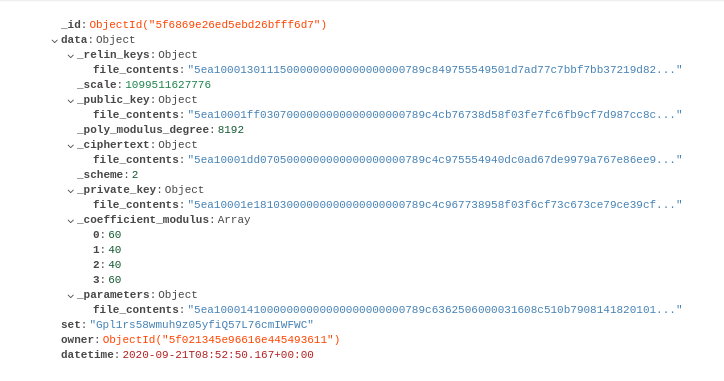
\includegraphics[width=0.5\linewidth]{data.png}
    \end{frame}

    \begin{frame}{Fully Homomorphic Encryption}
      \begin{columns}
        \begin{column}{0.5\textwidth}
          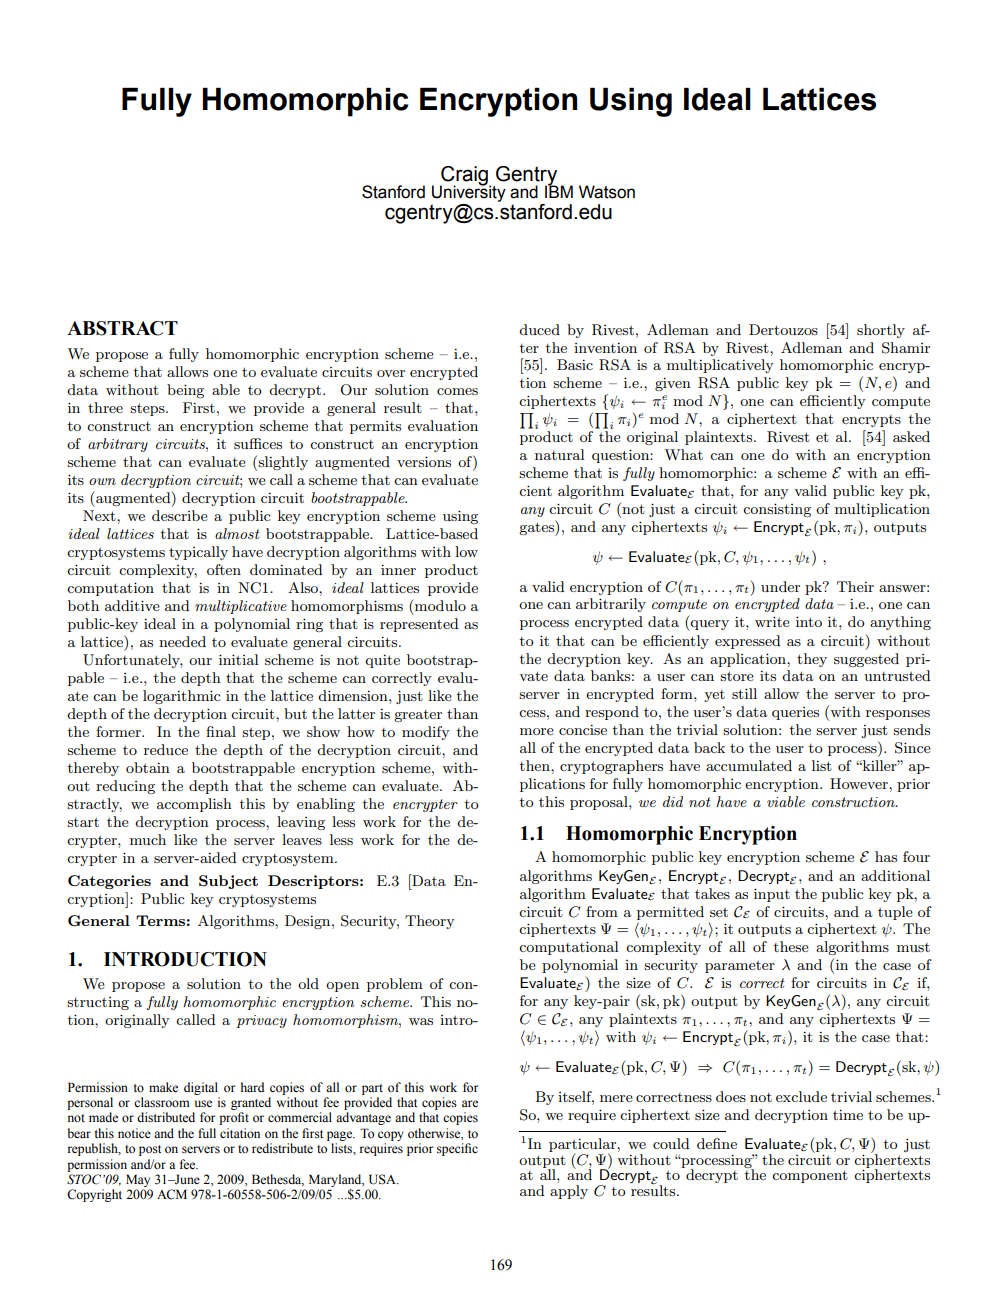
\includegraphics[width=0.8\linewidth]{gentry.png}
        \end{column}
        \begin{column}{0.5\textwidth}
          Second Column\\[.2cm]
          \begin{itemize}
            \item "Holy grail of encryption"
            \item Arbitrary computational depth on ciphertext
            \item Quantum decryption resistant ciphertext
            \item Abelian group operations \{+n,+(-n),*n\} on ciphertext
            \item Unable to compute non ableian operations such as division
          \end{itemize}
        \end{column}
      \end{columns}
    \end{frame}

    \begin{frame}{Deep Learning}
      \begin{columns}
        \begin{column}{0.5\textwidth}
          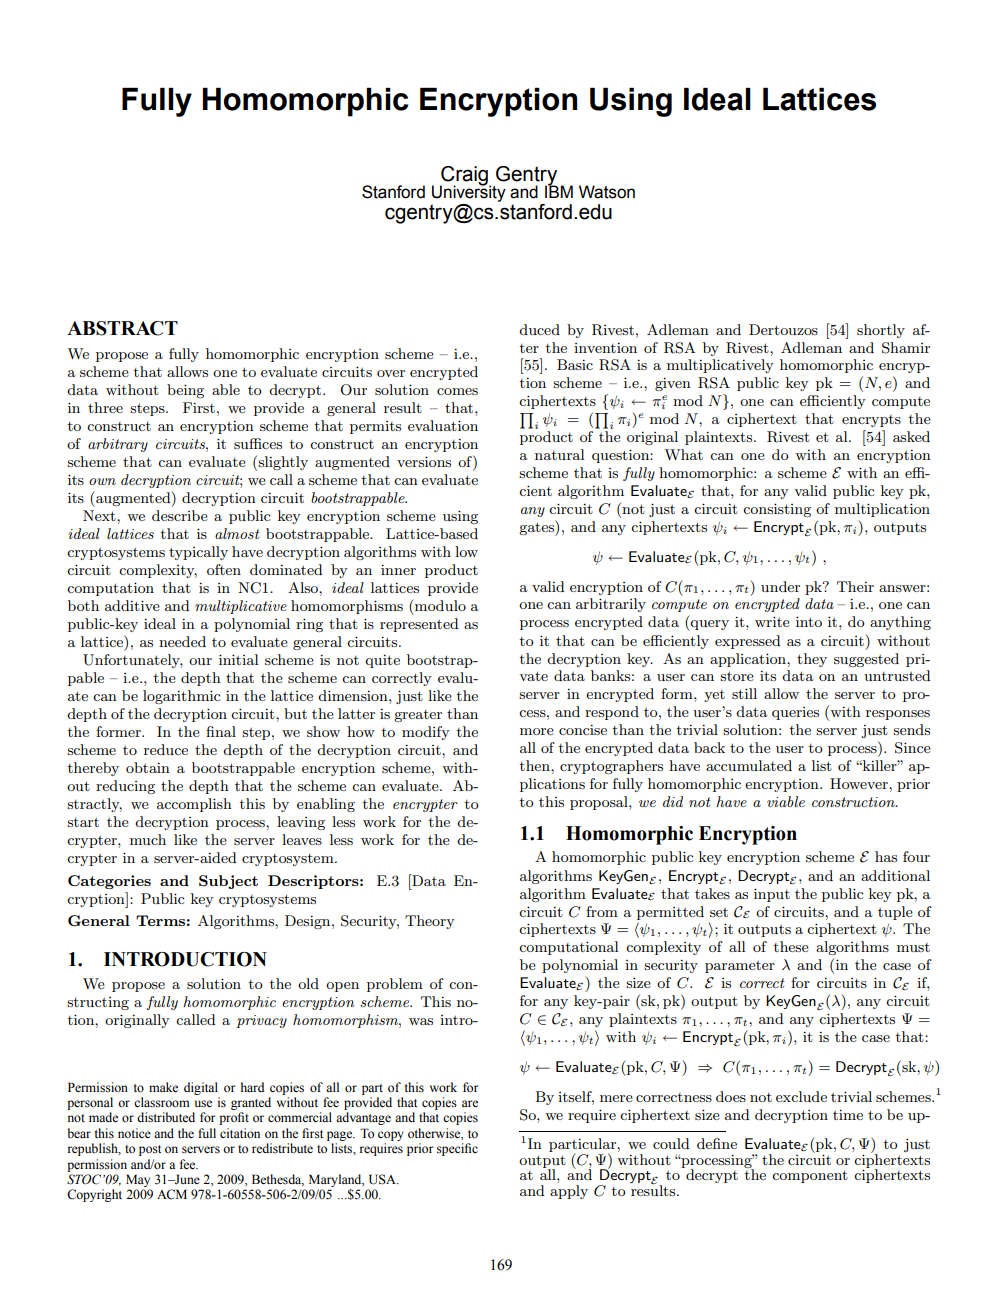
\includegraphics[width=0.8\linewidth]{gentry.png}
        \end{column}
        \begin{column}{0.5\textwidth}
          Second Column\\[.2cm]
          \begin{itemize}
            \item "Holy grail of encryption"
            \item Arbitrary computational depth on ciphertext
            \item Quantum decryption resistant ciphertext
            \item Abelian group operations ${+n,+(-n),*n}$ on ciphertext
            \item Unable to compute non ableian operations such as division
          \end{itemize}
        \end{column}
      \end{columns}
    \end{frame}

  \section{Methodology}

    \begin{frame}{Deep Learning $+$ Fully Homomorphic Encryption}

    \end{frame}

  \section{Results}

  \section{Summary}

    \begin{frame}{Conclusion}
      \begin{itemize}
        \item a
      \end{itemize}
    \end{frame}

  \section{Bibliography}

    \begin{frame}[allowframebreaks]
      \frametitle{References}
      \bibliographystyle{unsrt}
      \bibliography{./src/fhe.bib}%must have no space after ,
    \end{frame}

  \section{Appendix}

    \begin{figure}[allowframebreaks]
      \frametitle{Appendix}
    \end{figure}


\end{document}
